
The goal of our work is to extract opinions and sentiments about mobile applications from user reviews written in Thai. The work hopes to help Thai users assesss mobile application without needing to read all reviews and to also help Thai developers pinpoint where they can improve their software products. To achieve the goal, we employ 5 steps as follows: 1. Data Collection 2. Prepossessing 3. Sentiment Analysis 4. Topic Extraction 5. Summary as shown in Figure \ref{fig:approachFig}. 

\begin{figure}[h]
	\centering
	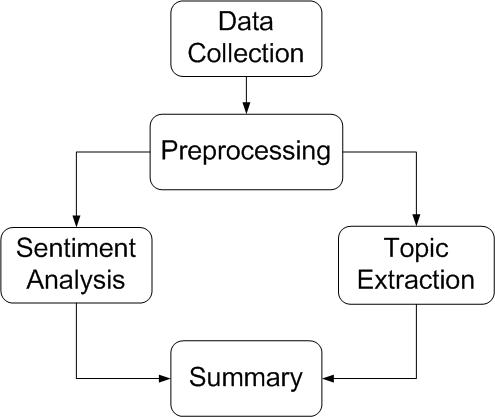
\includegraphics[width=.8\linewidth]{Process.jpg}
	\caption{Overview of approach}
	\label{fig:approachFig}
\end{figure}

We would like the entire process of analyzing raw user reviews to be automatic and accurate as much as possible, but it is not feasible to be 100\% automatic and accurate. To process raw user reviews, most of the process is done automatically but some parts need manual intervention. The following subsections describe these five steps and will also state whether the step is done automatically or manually. We also need to make some assumptions to make the process possible. For example, we assume that one sentence has one sentiment.

\subsection{Data Collection}

\begin{table}[h]
	\caption{Number of reviews in each application}
	\label{table:NoOfReview}
	\centering
	\begin{tabular}{|c|r|}
		\hline
		\textbf{Application} & \multicolumn{1}{|c|}{\textbf{No. of Reviews}} \\
		\hline
		Man Man & 1279\\
		\hline
		H-TV & 691\\
		\hline
		K-Mobile & 1055\\
		\hline
	\end{tabular}
\end{table}

\begin{table*}[h]
	\caption{Example of Reviews}
	\label{table:review}
	\centering
	\begin{tabular}{|l|l|l|c|c|}
		\hline
		\multicolumn{1}{|c|}{\textbf{Author}} &
		\multicolumn{1}{|c|}{\textbf{Title}} &
		\multicolumn{1}{|c|}{\textbf{Review}} &
		\multicolumn{1}{|c|}{\textbf{Rate}} &
		\multicolumn{1}{|c|}{\textbf{Date} (mm/dd/yyyy)}\\
		\hline
		{\selectlanguage{thai}โชคชัย มหาวงนันท์} & {\selectlanguage{thai}โชคชัย มหาวงศ์นันท์} & {\selectlanguage{thai}ใช้ได้ดีครับ} & 5&10/04/2015\\
		\hline
		bie slow life &  & {\selectlanguage{thai}พักหลังนี่อัพบ่อยนะครับ} & 4&09/19/2015\\
		\hline
		ornanohg Hongrrimon &  & {\selectlanguage{thai}ชอบค่ะใช้ง่าย มีตัวการ์ตูนให้ด้วย} & 5&09/20/2015\\
		\hline
		Terdsak chompusri &  & {\selectlanguage{thai}เรียบง่ายแต่ใช้ได้ดีจริงๆครับชอบมาก} & 5&09/22/2015\\
		\hline
		Worapote Panomauppatum & {\selectlanguage{thai}วรพจน์  พนมอุปถัมภ์} & {\selectlanguage{thai}ใช้ได้เยื่ยมมาก} & 5&09/25/2015\\
		\hline
		Nate Makboon & {\selectlanguage{thai}เนตร มากบุญ} & {\selectlanguage{thai}ดีมากครับ สะดวกดีแม่นสุดยอด} & 5&09/24/2015\\
		\hline
	\end{tabular}
\end{table*}


We have collected user reviews in Google Play Store from three mobile applications:
"{\selectlanguage{thai}แม่น แม่น}" or "Man Man" (a virtual keyboard), "H-TV" (online TV), "K-Mobile" (internet mobile banking). The user reviews collected are dated between February 2015 and August 2016. The number of user reviews collected for each application is shown in Table \ref{table:NoOfReview}. The information collected for each review includes author, title, detail, rate, and review date. Table \ref{table:review} shows examples of user reviews. A script is written to retrieve user reviews automatically from the Google Play Store website. The user reviews are then stored in a ...... database.

\subsection{Prepossessing}

After user reviews have been collected, the next step is to perform sentence segmentation, word segmentation and part-of-speech tagging. 

\subsubsection{sentence extraction}
One user review can contain several sentences expressing opinions about various aspects or features. 
Since we make an assumption that one sentence has one sentiment, we need to distinguish different sentences in the review. Thai writing however makes it difficult because there is no formal sentence boundary like a period or a question mark in Engish writing. Spaces in Thai language can mark the end of a sentence or the end of a clause. Therefore, we cannot simply use spaces to indicate the end of sentences. Although there are several researches focusing on breaking Thai text into sentences, there are no tools that can easily be used. We therefore perform sentence segmentation manually. Once a tool is available, it can be applied to make this pre-processing step easier. 

\subsubsection{word segmentation}
As mentioned in Section \ref{Background}, we used LexTo\cite{LexTo} from NECTEC to perform word segmentation. LexTo can segment words very well if words are spelled correctly. However, processing raw user reviews is difficult because of the informal language and slangs used in the reviews. There are also many spelling errors, either accidentally or intentionally to emphasize the meaning such as "{\selectlanguage{thai}มากกกกกก}", causing the tool to segment words incorrectly. 

To ease the problem, LexTo allows us to add new vocabulary into the tool. However, with too many slangs including new ones and too many variations of misspelled words, it is not practical to add all of these into the tool. Today, more and more texts to be analyzed are written informally. It is more practical to find an automatic approach to deal with this problem rather than manually correctly these words so that the word segmentation tool can perform entirely correctly. In our work, we have added some common slangs and common misspelled into the tool to increase accuracy but are not able to cover all slangs and mispelled words. This step is therefore more automatic with the cost of less accuracy.

\subsubsection{POS tagger}

We use the RDRPOStagger tool\cite{RDRPOSTagger} with the ORCHID corpus\cite{ORCHID} for POS tagging. Since some slang and mispelled words are segmented incorrectly, the POS tagger tags those words as "unknown". In the sentiment analysis and topic modeling steps, words tagged with nouns, verbs, and adjective/adverb are used to analyzed. In addition, since one word can be tagged with more than one POS, this POS annotation is used to identify various meanings of one word.

\subsection{Sentiment Analysis}
Once words in user reviews are tagged with parts of speech, sentiments in these reviews can be analyzed. Our work applies the lexicon-based approach. However, there is no resource that annotates each Thai word with sentiment scores. Therefore, the English SentiWordNet \cite{SentiWordNet} is used in combination with an electronic Thai-English dictionary called LEXiTRON \cite{LEXiTRON} developed by NECTEC.

To find score for each Thai word, our script automatically looks up in the LEXiTRON dictionary to retrieve its English word with the same part-of-speech tag. The next step is to look for sentiment score in SentiWordNet for the English word with the same POS. The sentiment score is between [-1,1] where negative number means negative sentiment and vice versa. Also, the higher the number means higher degree of negativity or positivity. Table \ref{table:Top10sentiword} shows examples of the sentiment scores. 

Besides assigning sentiment scores straightforwardly, further analysis is needed. For example, 
a word that is preceded with the word {\selectlanguage{thai}ไม่}, which means "no" or "not", will have its sentiment score flipped. In addition, some Thai words have more than one associated English words where these English words also have different sentiment scores. In this case, all sentiment scores are  averaged and then assigned to the Thai word. When sentiment scores are assigned to all nouns, verbs, adjectives, and adverbs in a sentence, the sentiment score for a sentence is calculated by averaging these sentiment scores.

Furthermore, we found that several negative sentences are assigned with positive score. Upon closer looks, we found a pattern in these sentences where there is a word {\selectlanguage{thai}ชอบ} preceding with negative verb such as {\selectlanguage{thai}แอพชอบล่มบ่อย}, which means the application often crashes. Since the word {\selectlanguage{thai}ชอบ} in Thai can mean "like" or if used in front of a verb it also means "often". Since the POS tool tags {\selectlanguage{thai}ชอบ} as a verb and the sentiment score comes out with a high positive number, this kind of sentences are therefore incorrectly assigned with positive numbers. We therefore eliminated the word {\selectlanguage{thai}ชอบ} that precedes a verb.


{\selectlanguage{thai}ชอบ} ..........GIVE EXAMPLE........


\begin{table}[h]
	\renewcommand{\arraystretch}{1.3}
	\caption{Top 10 sentiment of each word in Man Man app}
	\label{table:Top10sentiword}
	\centering
	\begin{tabular}{|c|c|c|c|}
		\hline
		\multicolumn{2}{|c|}{negative} &
		\multicolumn{2}{|c|}{positive}\\
		\hline
		word & sentiment & word & sentiment\\
		\hline
		{\selectlanguage{thai}ลบ} & -0.33621 & {\selectlanguage{thai}น่ารัก} & 0.21843\\
		\hline
		{\selectlanguage{thai}เสียดาย} & -0.33621 & {\selectlanguage{thai}รัก} & 0.21843\\
		\hline
		{\selectlanguage{thai}เกลียด} & -0.33621 & {\selectlanguage{thai}เพลิน} & 0.21843\\
		\hline
		{\selectlanguage{thai}ดุ} & -0.33621 & {\selectlanguage{thai}ดี} & 0.21843\\
		\hline
		{\selectlanguage{thai}สายตายาว} & -0.33621 & {\selectlanguage{thai}สวย} & 0.21843\\
		\hline
		{\selectlanguage{thai}ขยายตัว} & -0.33621 & {\selectlanguage{thai}สุดยอด} & 0.21843\\
		\hline
		{\selectlanguage{thai}ห่วย} & -0.33621 & {\selectlanguage{thai}มันส์} & 0.21843\\
		\hline
		{\selectlanguage{thai}ปวด} & -0.33621 & {\selectlanguage{thai}ไว} & 0.21843\\
		\hline
		{\selectlanguage{thai}เสียใจ} & -0.33621 & {\selectlanguage{thai}ชอบ} & 0.21843\\
		\hline
		{\selectlanguage{thai}ไม่ได้} & -0.33621 & {\selectlanguage{thai}สนุก} & 0.21843\\
		\hline
	\end{tabular}
\end{table}

\subsection{Topic or Feature Extraction}
In addition to sentiment analysis, we also want to pinpoint what features or topics users are talking about in the review. We use LDA for topic modeling. We supplied the user reviews to the LDA Python tool by using only nouns, verbs, adjectives, adverbs. We specify the number of topics to be 20 because we do not know exactly how many features users are talking about in the reviews.

We then choose topics with high probabilities and also choose words within the topics with high probabilities.

%not finish

\subsection{Summary}
After sentences are annotated with sentiment scores and features are extracted, we summarize the information to assign sentiment scores to the extracted features. Sentences containing words belonging to a topic are grouped together and their scores are averaged to assign sentiment scores to the topic. 

In addition, we also count how many sentencse with positive and negative scores for each topic so that developers can see in more details how much users like or dislike the features. 





